% Options for packages loaded elsewhere
\PassOptionsToPackage{unicode}{hyperref}
\PassOptionsToPackage{hyphens}{url}
\PassOptionsToPackage{dvipsnames,svgnames,x11names}{xcolor}
%
\documentclass[
  12pt,
  a4paper,
  DIV=11,
  numbers=noendperiod]{scrartcl}

\usepackage{amsmath,amssymb}
\usepackage{iftex}
\ifPDFTeX
  \usepackage[T1]{fontenc}
  \usepackage[utf8]{inputenc}
  \usepackage{textcomp} % provide euro and other symbols
\else % if luatex or xetex
  \usepackage{unicode-math}
  \defaultfontfeatures{Scale=MatchLowercase}
  \defaultfontfeatures[\rmfamily]{Ligatures=TeX,Scale=1}
\fi
\usepackage{lmodern}
\ifPDFTeX\else  
    % xetex/luatex font selection
  \setmainfont[]{Spectral}
  \setsansfont[]{Roboto}
  \setmonofont[]{Cascadia Code}
\fi
% Use upquote if available, for straight quotes in verbatim environments
\IfFileExists{upquote.sty}{\usepackage{upquote}}{}
\IfFileExists{microtype.sty}{% use microtype if available
  \usepackage[]{microtype}
  \UseMicrotypeSet[protrusion]{basicmath} % disable protrusion for tt fonts
}{}
\makeatletter
\@ifundefined{KOMAClassName}{% if non-KOMA class
  \IfFileExists{parskip.sty}{%
    \usepackage{parskip}
  }{% else
    \setlength{\parindent}{0pt}
    \setlength{\parskip}{6pt plus 2pt minus 1pt}}
}{% if KOMA class
  \KOMAoptions{parskip=half}}
\makeatother
\usepackage{xcolor}
\usepackage[top=20mm,left=20mm,right=20mm,bottom=20mm,heightrounded]{geometry}
\setlength{\emergencystretch}{3em} % prevent overfull lines
\setcounter{secnumdepth}{5}
% Make \paragraph and \subparagraph free-standing
\ifx\paragraph\undefined\else
  \let\oldparagraph\paragraph
  \renewcommand{\paragraph}[1]{\oldparagraph{#1}\mbox{}}
\fi
\ifx\subparagraph\undefined\else
  \let\oldsubparagraph\subparagraph
  \renewcommand{\subparagraph}[1]{\oldsubparagraph{#1}\mbox{}}
\fi


\providecommand{\tightlist}{%
  \setlength{\itemsep}{0pt}\setlength{\parskip}{0pt}}\usepackage{longtable,booktabs,array}
\usepackage{calc} % for calculating minipage widths
% Correct order of tables after \paragraph or \subparagraph
\usepackage{etoolbox}
\makeatletter
\patchcmd\longtable{\par}{\if@noskipsec\mbox{}\fi\par}{}{}
\makeatother
% Allow footnotes in longtable head/foot
\IfFileExists{footnotehyper.sty}{\usepackage{footnotehyper}}{\usepackage{footnote}}
\makesavenoteenv{longtable}
\usepackage{graphicx}
\makeatletter
\def\maxwidth{\ifdim\Gin@nat@width>\linewidth\linewidth\else\Gin@nat@width\fi}
\def\maxheight{\ifdim\Gin@nat@height>\textheight\textheight\else\Gin@nat@height\fi}
\makeatother
% Scale images if necessary, so that they will not overflow the page
% margins by default, and it is still possible to overwrite the defaults
% using explicit options in \includegraphics[width, height, ...]{}
\setkeys{Gin}{width=\maxwidth,height=\maxheight,keepaspectratio}
% Set default figure placement to htbp
\makeatletter
\def\fps@figure{htbp}
\makeatother
\newlength{\cslhangindent}
\setlength{\cslhangindent}{1.5em}
\newlength{\csllabelwidth}
\setlength{\csllabelwidth}{3em}
\newlength{\cslentryspacingunit} % times entry-spacing
\setlength{\cslentryspacingunit}{\parskip}
\newenvironment{CSLReferences}[2] % #1 hanging-ident, #2 entry spacing
 {% don't indent paragraphs
  \setlength{\parindent}{0pt}
  % turn on hanging indent if param 1 is 1
  \ifodd #1
  \let\oldpar\par
  \def\par{\hangindent=\cslhangindent\oldpar}
  \fi
  % set entry spacing
  \setlength{\parskip}{#2\cslentryspacingunit}
 }%
 {}
\usepackage{calc}
\newcommand{\CSLBlock}[1]{#1\hfill\break}
\newcommand{\CSLLeftMargin}[1]{\parbox[t]{\csllabelwidth}{#1}}
\newcommand{\CSLRightInline}[1]{\parbox[t]{\linewidth - \csllabelwidth}{#1}\break}
\newcommand{\CSLIndent}[1]{\hspace{\cslhangindent}#1}

\addtokomafont{disposition}{\rmfamily}
\KOMAoption{captions}{tableheading}
\makeatletter
\makeatother
\makeatletter
\makeatother
\makeatletter
\@ifpackageloaded{caption}{}{\usepackage{caption}}
\AtBeginDocument{%
\ifdefined\contentsname
  \renewcommand*\contentsname{Table of contents}
\else
  \newcommand\contentsname{Table of contents}
\fi
\ifdefined\listfigurename
  \renewcommand*\listfigurename{List of Figures}
\else
  \newcommand\listfigurename{List of Figures}
\fi
\ifdefined\listtablename
  \renewcommand*\listtablename{List of Tables}
\else
  \newcommand\listtablename{List of Tables}
\fi
\ifdefined\figurename
  \renewcommand*\figurename{Figure}
\else
  \newcommand\figurename{Figure}
\fi
\ifdefined\tablename
  \renewcommand*\tablename{Table}
\else
  \newcommand\tablename{Table}
\fi
}
\@ifpackageloaded{float}{}{\usepackage{float}}
\floatstyle{ruled}
\@ifundefined{c@chapter}{\newfloat{codelisting}{h}{lop}}{\newfloat{codelisting}{h}{lop}[chapter]}
\floatname{codelisting}{Listing}
\newcommand*\listoflistings{\listof{codelisting}{List of Listings}}
\makeatother
\makeatletter
\@ifpackageloaded{caption}{}{\usepackage{caption}}
\@ifpackageloaded{subcaption}{}{\usepackage{subcaption}}
\makeatother
\makeatletter
\@ifpackageloaded{tcolorbox}{}{\usepackage[skins,breakable]{tcolorbox}}
\makeatother
\makeatletter
\@ifundefined{shadecolor}{\definecolor{shadecolor}{rgb}{.97, .97, .97}}
\makeatother
\makeatletter
\makeatother
\makeatletter
\makeatother
\ifLuaTeX
  \usepackage{selnolig}  % disable illegal ligatures
\fi
\IfFileExists{bookmark.sty}{\usepackage{bookmark}}{\usepackage{hyperref}}
\IfFileExists{xurl.sty}{\usepackage{xurl}}{} % add URL line breaks if available
\urlstyle{same} % disable monospaced font for URLs
\hypersetup{
  pdftitle={The Impact of Terrain on Cycle Hire Journey Frequency},
  pdfauthor={Soki Kimura},
  colorlinks=true,
  linkcolor={blue},
  filecolor={Maroon},
  citecolor={Blue},
  urlcolor={Blue},
  pdfcreator={LaTeX via pandoc}}

\title{The Impact of Terrain on Cycle Hire Journey Frequency}
\author{Soki Kimura}
\date{}

\begin{document}
\maketitle
\ifdefined\Shaded\renewenvironment{Shaded}{\begin{tcolorbox}[interior hidden, borderline west={3pt}{0pt}{shadecolor}, boxrule=0pt, enhanced, sharp corners, breakable, frame hidden]}{\end{tcolorbox}}\fi

\hypertarget{introduction}{%
\section{Introduction}\label{introduction}}

The rapid spread of cycle hire schemes impact the transport system in
cities worldwide, increasing the share of cycling and public transport
usage, lowering greenhouse gas emissions, and improving public health
(DeMaio, 2009). Since its first implication in Amsterdam in the 1960s,
the system has seen technological and methodological improvements over
time. The modern system equipped with telecommunication technology has
enabled casual usages between different stations, encouraging short,
high-frequency and one-way journeys(Beroud and Anaya, 2012; Beecham,
2015). The London Cycle Hire Scheme (LCHS), known as the Santander
Cycles, is one of these systems. In service since 2010 (Li \emph{et
al.}, 2019), it has 800 docking stations within central London
(Transport for London, 2023b).

\hypertarget{literature-review}{%
\section{Literature Review}\label{literature-review}}

The detailed datasets of cycle hire schemes such as LCHS around the
world has enabled analysis for cycling behaviour from many aspects.
Gebhart and Noland (2014) has found uncomfortable weather conditions
including cold weather, precipitation, and high humidity reduces
bikeshare usage in Washington DC. Wood, Slingsby and Dykes (2011)
explored the visualisation of journeys taken by the LCHS, illustrating
two major patterns of usage: leisure usage often seen near Royal Parks
and commuting to and from major train stations in peak hours.
Accessibility by other public transport modes also impact the usage of
bicycle hire schemes (Gebhart and Noland, 2014).

Meanwhile, research on the relationship between cycling behaviour and
the physical environment is limited (Heinen, Wee and Maat, 2010). A
small number of past researches (Rodrı́guez and Joo, 2004; Parkin,
Wardman and Page, 2008) show that hilliness has a negative impact on
cycling. The terrain is quantified in different ways, one segmenting the
actual routes surveyed, while the other calculates the average
percentage of slope using raster data.

Drawing on these two streams, this report has conducted an anlysis on
the unexplored relationship between cycle hire scheme usage behaviour
and the physical environment.

\hypertarget{research-question}{%
\section{Research Question}\label{research-question}}

Does the slope of the physical environment impact the number of cycle
hire trips?

\hypertarget{hypothesis}{%
\section{Hypothesis}\label{hypothesis}}

We hypothesised there will be less journeys under hilly conditions, and
tested the following two perspectives:

\begin{enumerate}
\def\labelenumi{\arabic{enumi}.}
\tightlist
\item
  Docking stations located in lower elevations have more arriving
  journeys than departures, while stations with high elevation being the
  opposite.
\item
  There will be a smaller number of trips for origin-destination pairs
  requiring uphill travel.
\end{enumerate}

\hypertarget{data}{%
\section{Data}\label{data}}

\hypertarget{data-sources}{%
\subsection{Data Sources}\label{data-sources}}

The LCHS data published by Transport for London (TfL) is used (Transport
for London, 2023b, 2023a), which has the following attributes:

\begin{longtable}[]{@{}
  >{\raggedright\arraybackslash}p{(\columnwidth - 2\tabcolsep) * \real{0.5000}}
  >{\raggedright\arraybackslash}p{(\columnwidth - 2\tabcolsep) * \real{0.5000}}@{}}
\caption{List of attributes available for LCHS data}\tabularnewline
\toprule\noalign{}
\begin{minipage}[b]{\linewidth}\raggedright
Dataset
\end{minipage} & \begin{minipage}[b]{\linewidth}\raggedright
Attributes
\end{minipage} \\
\midrule\noalign{}
\endfirsthead
\toprule\noalign{}
\begin{minipage}[b]{\linewidth}\raggedright
Dataset
\end{minipage} & \begin{minipage}[b]{\linewidth}\raggedright
Attributes
\end{minipage} \\
\midrule\noalign{}
\endhead
\bottomrule\noalign{}
\endlastfoot
Docking Station Data & location, name, ID, number of docks per
station \\
Journeys Data & Start and end station data (ID, name), date and time,
duration, type of cycle (conventional or e-cycle) \\
\end{longtable}

The other datasets used for analysis, and a map of docking stations
merged with its height are shown below.

\begin{longtable}[]{@{}
  >{\raggedright\arraybackslash}p{(\columnwidth - 6\tabcolsep) * \real{0.2500}}
  >{\raggedright\arraybackslash}p{(\columnwidth - 6\tabcolsep) * \real{0.2500}}
  >{\raggedright\arraybackslash}p{(\columnwidth - 6\tabcolsep) * \real{0.2500}}
  >{\raggedright\arraybackslash}p{(\columnwidth - 6\tabcolsep) * \real{0.2500}}@{}}
\caption{List of datasets used for additional
information}\tabularnewline
\toprule\noalign{}
\begin{minipage}[b]{\linewidth}\raggedright
\end{minipage} & \begin{minipage}[b]{\linewidth}\raggedright
Elevation Data
\end{minipage} & \begin{minipage}[b]{\linewidth}\raggedright
Accessibility to Public Transport
\end{minipage} & \begin{minipage}[b]{\linewidth}\raggedright
Geometries
\end{minipage} \\
\midrule\noalign{}
\endfirsthead
\toprule\noalign{}
\begin{minipage}[b]{\linewidth}\raggedright
\end{minipage} & \begin{minipage}[b]{\linewidth}\raggedright
Elevation Data
\end{minipage} & \begin{minipage}[b]{\linewidth}\raggedright
Accessibility to Public Transport
\end{minipage} & \begin{minipage}[b]{\linewidth}\raggedright
Geometries
\end{minipage} \\
\midrule\noalign{}
\endhead
\bottomrule\noalign{}
\endlastfoot
Dataset & LIDAR Composite Digital Terrain Model (DTM) (Environment
Agency, 2023) & Access Index (AI) (Transport for London, 2015b) &
Statistical boundaries (Greater London Authority, 2014), Congestion
Charge boundaries (Greater London Authority, 2019) \\
Specifications & Resolution: 2 m & Basis for the Public Transport
Accessibility Levels (PTAL) (Transport for London, 2015a).
\(\text{AI}<2.5\) will be lowest PTAL (1a), \(\text{AI}>40\) classified
as highest (6b) & Downloaded via London Datastore \\
\end{longtable}

\begin{figure}

{\centering 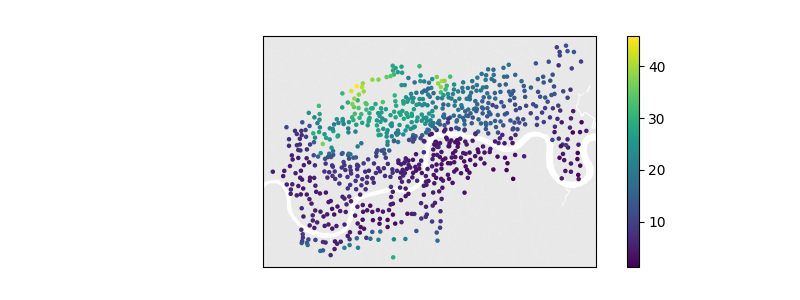
\includegraphics{img/docking_stations.png}

}

\caption{The location and elevation of docking stations in London}

\end{figure}

\hypertarget{summary-of-data}{%
\subsection{Summary of data}\label{summary-of-data}}

The scope of analysis is the journeys taken on the LCHS from December
2022 to November 2023, the most recent one-year period where data is
available. There is a total of 8,414,631 journeys taken during this
period.

\begin{longtable}[]{@{}lrrr@{}}
\caption{Characteristics of journeys made by the LCHS}\tabularnewline
\toprule\noalign{}
Statistics & Classic Cycles & E-cycles & Total \\
\midrule\noalign{}
\endfirsthead
\toprule\noalign{}
Statistics & Classic Cycles & E-cycles & Total \\
\midrule\noalign{}
\endhead
\bottomrule\noalign{}
\endlastfoot
Number of Trips & 7,808,234 & 606,397 & 8,414,631 \\
Mean Travelled Distance {[}m{]} & 2279.41 & 3124.62 & 2340.32 \\
Mean Height Difference of Travel {[}m{]} & -0.23 & -0.07 & -0.22 \\
\end{longtable}

The negative average in height difference indicate downhill travel is
slightly preferred over their uphill counterparts. A one-sample t-test
shows this value is significant compared to a mean of 0.

Journeys by e-cycles are longer and have less height difference compared
to conventional cycles, suggesting physically demanding journeys are
avoided by classic cycle users. Focusing on journeys made by classic
cycles, this is the hypothesis we have addressed.

\hypertarget{methodology}{%
\section{Methodology}\label{methodology}}

This research is conducted in two parts. We have first analysed
individual docking stations, followed by an analysis on
origin-destination combinations. An extensive literature review by
Heinen, Wee and Maat (2010) has summarised factors affecting cycling
behaviour, and based on the data availability we have considered the
following variables:

\begin{itemize}
\tightlist
\item
  distance of journey (average distance between docking stations)
\item
  population density of MSOA
\item
  access to public transport (average AI value of stations)
\item
  number of docking stations in MSOA
\item
  direction of journey
\end{itemize}

\hypertarget{analyse-the-usage-of-individual-docking-stations}{%
\subsection{Analyse the usage of individual docking
stations}\label{analyse-the-usage-of-individual-docking-stations}}

The ratio of departing journeys compared to arriving journeys
(hereinafter ``DA ratio'') was tested against elevation and other
characteristics of the station in a linear regression model. The number
of ports per station, the location of station relative to the central
zone, the AI, and the population density of MSOA were considered as
additional factors.

\hypertarget{summarizing-the-data-into-origin-destination-pairs}{%
\subsection{Summarizing the data into Origin-Destination
pairs}\label{summarizing-the-data-into-origin-destination-pairs}}

We have summarised the data by grouping them by their origin and
destination. MSOAs are used as the unit of analysis in order to reduce
the size of the matrix. There are 160 MSOAs where LCHS operates,
therefore the summarised dataset includes 25,600 rows of data. By
removing journeys that start and finish within the same MSOA, we have
25,440 rows of data for analysis.

\hypertarget{analysis-of-variables}{%
\subsubsection{Analysis of variables}\label{analysis-of-variables}}

The scatter plot between the distance and the journeys is shown below,
along with a semi-log plot and a log-log plot.

\begin{figure}

{\centering 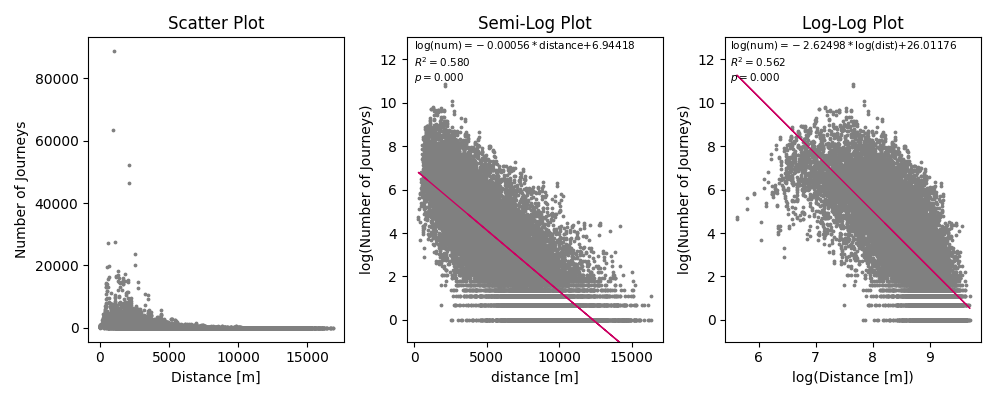
\includegraphics{img/scatter_MSOA.png}

}

\caption{Correlation of Distance and Number of Journeys between MSOAs}

\end{figure}

The log plot resembles a linear correlation, while the log-log plot has
an upward convex. Thus, the relationship between distance and number of
journeys follow an exponential relation. Assuming the other variables
have a linear relationship, the model we will use to estimate the number
of journeys is as follows:

\[
y = \alpha_\text{dist} \exp(\beta_\text{dist} x_\text{dist}) + \sum_i{\beta_ix_i} + \alpha
\]

\begin{itemize}
\tightlist
\item
  \(x_{\text{dist}}\): distance of journey
\item
  \(\beta_\text{dist}\): coefficient for exponential law (slope of
  semi-log regression line)
\item
  \(\alpha_\text{dist}\): constant for exponential law (intercept of
  semi-log regression line)
\item
  \(x_i\): other explanatory variables
\item
  \(\alpha\): constant for linear regression
\item
  \(\beta_i\): coefficients for linear regression
\end{itemize}

By considering \(\exp(\beta_\text{dist} x_\text{dist})\) as one variable
\texttt{distance\_exp} and \(\alpha_\text{dist}\) as its coefficient,
the algorithm for a multiple linear regression can be utilised for our
proposed model.

\hypertarget{results}{%
\section{Results}\label{results}}

\hypertarget{analysis-of-individual-points}{%
\subsection{Analysis of Individual
Points}\label{analysis-of-individual-points}}

The relationship between the elevation and cycling activities is shown
below. The DA ratio has a linear correlation with the elevation, and is
statistically significant explaining 11.0 \% of the variance in the DA
ratio.

\begin{figure}

{\centering 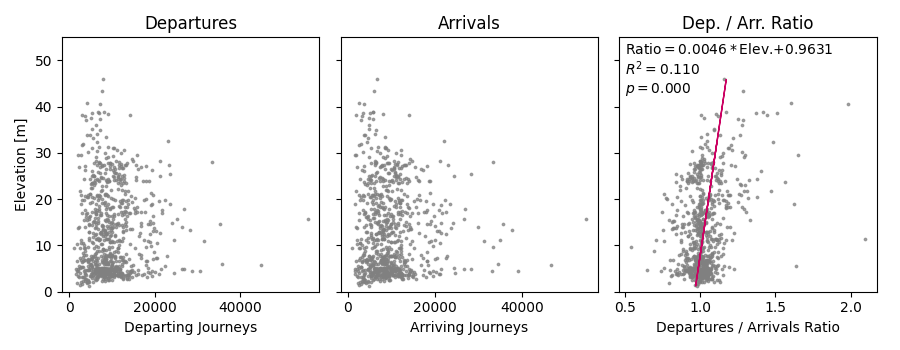
\includegraphics{img/elev_scatter.png}

}

\caption{Relationship between elevation and docking station usage}

\end{figure}

We will consider the multiple linear regression for the DA ratio. The
Pearson's correlation matrix below shows no sign of multicollinearity,
and a linear correlation between the independent variable and the
dependent variables.

\begin{figure}

{\centering 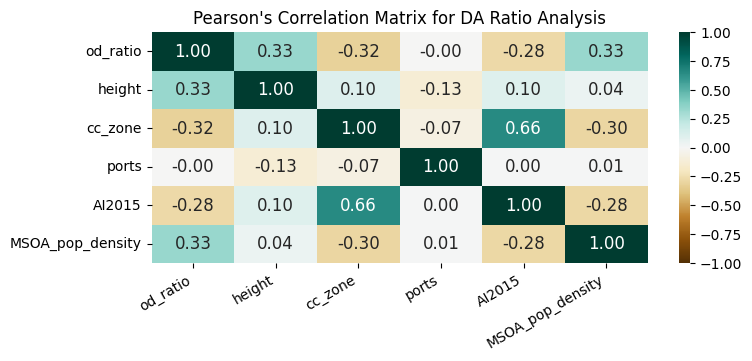
\includegraphics{img/cor_matrix_DA.png}

}

\caption{Pearson's correlation matrix for DA ratio analysis}

\end{figure}

The results of the regression model is as follows.

\begin{longtable}[]{@{}lrrrr@{}}
\caption{Results of the regression model. Adjusted R-squared value:
\(R^2 = 0.286\). The height, location, accessibility and the population
density are statistically significant, while the number of ports per
station is insignificant.}\tabularnewline
\toprule\noalign{}
Variable & Coefficient & Standard Error & \(t\) & \(P > |t|\) \\
\midrule\noalign{}
\endfirsthead
\toprule\noalign{}
Variable & Coefficient & Standard Error & \(t\) & \(P > |t|\) \\
\midrule\noalign{}
\endhead
\bottomrule\noalign{}
\endlastfoot
Constant & 0.9246 & 0.018 & 52.034 & 0.000 \\
\texttt{Height} & 0.0049 & 0.000 & 11.783 & 0.000 \\
\texttt{cc\_zone} & -0.0567 & 0.011 & -5.268 & 0.000 \\
\texttt{ports} & 0.0003 & 0.000 & 0.794 & 0.427 \\
\texttt{AI2015} & -0.0005 & 0.000 & -2.757 & 0.006 \\
\texttt{MSOA\_pop\_density} & 4.6302 & 0.660 & 7.011 & 0.000 \\
\end{longtable}

The factors that lead to more departures than arrivals are the elevation
and the population density of the area, while locating in the central
zone and the accessibility to public transport lead to more arriving
journeys. A 1 m rise in elevation leads to a 0.5 \% increase in
departures compared to arrivals. stations in the highest PTAL band (AI
\textgreater{} 40) will have 2 \% more arrivals than departures compared
to the lowest band (AI \textless{} 2.5).

\begin{figure}

{\centering 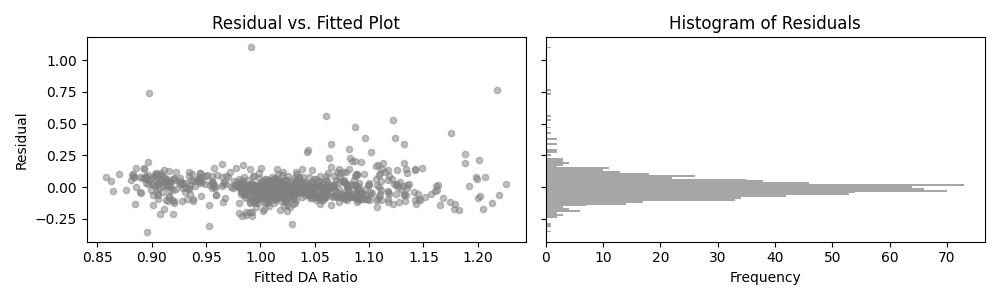
\includegraphics{img/residual_DA.png}

}

\caption{Residual vs.~Fitted Plot and the histogram of residuals for the
model. The homoscedasticity and the normal distribution of errors can be
confirmed.}

\end{figure}

\hypertarget{analysis-of-the-origin-destination-flow}{%
\subsection{Analysis of the origin-destination
flow}\label{analysis-of-the-origin-destination-flow}}

Now, we will analyse the flow of cycles using an origin-destination
analysis. The correlation matrix is shown as follows:

\begin{figure}

{\centering 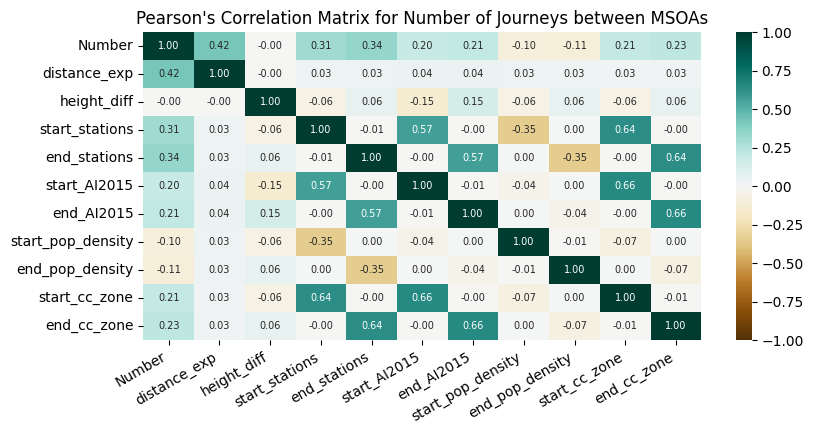
\includegraphics{img/cor_matrix_MSOA.png}

}

\caption{Pearson's correlation matrix for OD analysis}

\end{figure}

There is a collinearity between the number of stations per area, the
accessibility by public transport, and whether the docks are in the
central area, although this is below the threshold of 5 for a VIF
analysis. The results of the regression model is as follows.

\begin{longtable}[]{@{}lrrrr@{}}
\caption{Results of the regression model. Adjusted R-squared value:
\(R^2 = 0.373\). Distance, number of stations and the population density
are significant. The difference in height, along with the relationship
with the central zone is not a significant factor. AI of destination is
statistically significant, while AI of origin is not
(\(p > 0.05\)).}\tabularnewline
\toprule\noalign{}
Variable & Coefficient & Standard Error & \(t\) & \(P > |t|\) \\
\midrule\noalign{}
\endfirsthead
\toprule\noalign{}
Variable & Coefficient & Standard Error & \(t\) & \(P > |t|\) \\
\midrule\noalign{}
\endhead
\bottomrule\noalign{}
\endlastfoot
Constant & -552.5421 & 28.093 & -19.668 & 0.000 \\
\texttt{distance\_exp} & 2.7091 & 0.034 & 80.581 & 0.000 \\
\texttt{height\_diff} & -0.4716 & 0.394 & -1.196 & 0.232 \\
\texttt{start\_stations} & 57.9386 & 1.517 & 38.186 & 0.000 \\
\texttt{end\_stations} & 63.3330 & 1.517 & 41.741 & 0.000 \\
\texttt{start\_AI2015} & 0.6236 & 0.330 & 1.887 & 0.059 \\
\texttt{end\_AI2015} & 0.6825 & 0.330 & 2.065 & 0.039 \\
\texttt{start\_pop\_density} & -0.0026 & 0.001 & -2.569 & 0.010 \\
\texttt{end\_pop\_density} & -0.0037 & 0.001 & -3.675 & 0.000 \\
\texttt{start\_cc\_zone} & 25.3524 & 22.087 & 1.148 & 0.251 \\
\texttt{end\_cc\_zone} & 26.5992 & 22.087 & 1.204 & 0.228 \\
\end{longtable}

The model shows that there will be more travel between MSOAs if the
distance between the MSOAs are smaller, there are more stations within
each MSOA, or the population density is smaller.

\hypertarget{discussion}{%
\section{Discussion}\label{discussion}}

\hypertarget{the-impact-of-elevation}{%
\subsection{The impact of elevation}\label{the-impact-of-elevation}}

From the results, we can conclude that there is some relationship
between elevation and LCHS journeys. With focus on the individual
stations, stations located in elevated areas see more departures than
arrivals, which aligns with previous research and empirical observations
where an uphill journey has a negative impact on cycling. On the other
hand, the frequency of travel between MSOAs are not impacted by the
relative difference in their height.

The first point of discussion is that the relative height difference may
not be representing hilliness that negatively impacts cycling,
presenting a limitation of this research. Hills encountered en route,
the steepness of slope, and the general hilliness of the terrain are not
considered, which the methodology to quantify and the correlation with
frequency are both potential fields of further research.

The second possibility is that slope may be irrelavant for the overall
route selection. London is a flat city with over 75 \% of the stations
located between 0-20 m in elevation, and the small difference may not be
enough to alter mode choice in the macro scale. The difference observed
in the scale of individual ports may be caused by choice within the
area, where cyclists prefer departing from high stations but return at
nearby stations with lower elevation. Further analysis, considering
intra-MSOA differences should be conducted to confirm.

\hypertarget{other-factors-influencing-frequency}{%
\subsection{Other factors influencing
frequency}\label{other-factors-influencing-frequency}}

Through this research, other decisive factors affecting cycling
behaviour were discovered. Closer distances between areas saw more
journeys between them, which aligns with previous literature. The
negative correlation between population density may indicate usage is
more frequent in commercial areas than in residential areas. The
positive correlation between public transport accessibility for the
destination and cycling behaviour indicate bike-and-ride usage is
becoming common, which merits public transport users by reducing
door-to-door travel time (Martens, 2007). With the AI at the origin not
being significant, a \emph{ride-and-bike} behaviour seems to be less
common than cycling to public transport.

Interestingly, some factors triggering assymetry among outbound and
return trips have been discovered. High population density leads to more
departures, while being in the central zone increases arrivals. This may
indicate Londoners cycle on their way to the city centre, but use other
transport modes on their way back. The reasons, whether it might be the
darkness as suggested by Stinson and Bhat (2004), influence of alcohol,
or simply not wanting to engage in cycling after a long day, is a
potential area for future exploration.

\hypertarget{limitations}{%
\subsection{Limitations}\label{limitations}}

This research has not considered all factors that may influence cycling
behaviour, such as socio-economic factors, infrastructure, and weather.
The variables may be proxies of the actual dominant conditions, in which
case my discussions may be drawing incorrect conclusions. The journeys
by classic cycles on LCHS may not be the representation of the cycling
behaviour in London as a whole, which does not take into consideration
private cycles, e-scooters, and other bicycle hire schemes.

\hypertarget{conclusion}{%
\section{Conclusion}\label{conclusion}}

In this research, the correlation between elevation of individual
docking stations and departure-arrival ratio has shown uphill travels
have negative impact on cycling behaviour, although this pattern could
not be observed when considering the macro-scale origin-destination
journey frequency. The field of studying cycling behaviour through cycle
hire data is growing rapidly (Beecham, 2015), and further research is
expected for the better understanding of the effect of the physical
environment on cycle hire flows.

\hypertarget{reference}{%
\section*{Reference}\label{reference}}
\addcontentsline{toc}{section}{Reference}

\hypertarget{refs}{}
\begin{CSLReferences}{0}{0}
\leavevmode\vadjust pre{\hypertarget{ref-beecham2015}{}}%
Beecham, R. (2015) {`Using {Bikeshare} {Datasets} to {Improve} {Urban}
{Cycling} {Experience} and {Research} {Urban} {Cycling} {Behaviour}'},
in Gerike, R. and Parkin, J. (eds). Farnham: Ashgate, pp. 267--283.
Available at:
\url{https://www.crcpress.com/Cycling-Futures-From-Research-into-Practice/Gerike-Parkin/p/book/9781138546868}
(Accessed: 30 November 2023).

\leavevmode\vadjust pre{\hypertarget{ref-beroud2012}{}}%
Beroud, B. and Anaya, E. (2012) {`Private {Interventions} in a {Public}
{Service}: {An} {Analysis} of {Public} {Bicycle} {Schemes}'}, in Parkin,
J. (ed.) \emph{Cycling and {Sustainability}}. Emerald Group Publishing
Limited (Transport and {Sustainability}), pp. 269--301. doi:
\href{https://doi.org/10.1108/S2044-9941(2012)0000001013}{10.1108/S2044-9941(2012)0000001013}.

\leavevmode\vadjust pre{\hypertarget{ref-demaio2009}{}}%
DeMaio, P. (2009) {`Bike-sharing: {History}, {Impacts}, {Models} of
{Provision}, and {Future}'}, \emph{Journal of Public Transportation},
12(4), pp. 41--56. doi:
\href{https://doi.org/10.5038/2375-0901.12.4.3}{10.5038/2375-0901.12.4.3}.

\leavevmode\vadjust pre{\hypertarget{ref-environmentagency2023}{}}%
Environment Agency (2023) {`{LIDAR} {Composite} {Digital} {Terrain}
{Model} ({DTM}) 2m'}. Available at:
\url{https://environment.data.gov.uk/survey} (Accessed: 29 December
2023).

\leavevmode\vadjust pre{\hypertarget{ref-gebhart2014}{}}%
Gebhart, K. and Noland, R. B. (2014) {`The impact of weather conditions
on bikeshare trips in {Washington}, {DC}'}, \emph{Transportation},
41(6), pp. 1205--1225. doi:
\href{https://doi.org/10.1007/s11116-014-9540-7}{10.1007/s11116-014-9540-7}.

\leavevmode\vadjust pre{\hypertarget{ref-greaterlondonauthority2014}{}}%
Greater London Authority (2014) {`Statistical {GIS} {Boundary} {Files}
for {London} - {London} {Datastore}'}. Available at:
\url{https://data.london.gov.uk/dataset/statistical-gis-boundary-files-london}
(Accessed: 5 January 2024).

\leavevmode\vadjust pre{\hypertarget{ref-greaterlondonauthority2019}{}}%
Greater London Authority (2019) {`Ultra {Low} {Emissions} {Zone} 2019 -
{London} {Datastore}'}. Available at:
\url{https://data.london.gov.uk/dataset/ultra_low_emissions_zone}
(Accessed: 5 January 2024).

\leavevmode\vadjust pre{\hypertarget{ref-heinen2010}{}}%
Heinen, E., Wee, B. van and Maat, K. (2010) {`Commuting by {Bicycle}:
{An} {Overview} of the {Literature}'}, \emph{Transport Reviews}, 30(1),
pp. 59--96. doi:
\href{https://doi.org/10.1080/01441640903187001}{10.1080/01441640903187001}.

\leavevmode\vadjust pre{\hypertarget{ref-li2019}{}}%
Li, H. \emph{et al.} (2019) {`Effects of dockless bike-sharing systems
on the usage of the {London} {Cycle} {Hire}'}, \emph{Transportation
Research Part A: Policy and Practice}, 130, pp. 398--411. doi:
\href{https://doi.org/10.1016/j.tra.2019.09.050}{10.1016/j.tra.2019.09.050}.

\leavevmode\vadjust pre{\hypertarget{ref-martens2007}{}}%
Martens, K. (2007) {`Promoting bike-and-ride: {The} {Dutch}
experience'}, \emph{Transportation Research Part A: Policy and
Practice}, 41(4), pp. 326--338. doi:
\href{https://doi.org/10.1016/j.tra.2006.09.010}{10.1016/j.tra.2006.09.010}.

\leavevmode\vadjust pre{\hypertarget{ref-parkin2008}{}}%
Parkin, J., Wardman, M. and Page, M. (2008) {`Estimation of the
determinants of bicycle mode share for the journey to work using census
data'}, \emph{Transportation}, 35(1), pp. 93--109. doi:
\href{https://doi.org/10.1007/s11116-007-9137-5}{10.1007/s11116-007-9137-5}.

\leavevmode\vadjust pre{\hypertarget{ref-rodriguez2004}{}}%
Rodrı́guez, D. A. and Joo, J. (2004) {`The relationship between
non-motorized mode choice and the local physical environment'},
\emph{Transportation Research Part D: Transport and Environment}, 9(2),
pp. 151--173. doi:
\href{https://doi.org/10.1016/j.trd.2003.11.001}{10.1016/j.trd.2003.11.001}.

\leavevmode\vadjust pre{\hypertarget{ref-stinson2004}{}}%
Stinson, M. A. and Bhat, C. R. (2004) {`Frequency of {Bicycle}
{Commuting}: {Internet}-{Based} {Survey} {Analysis}'},
\emph{Transportation Research Record}, 1878(1), pp. 122--130. doi:
\href{https://doi.org/10.3141/1878-15}{10.3141/1878-15}.

\leavevmode\vadjust pre{\hypertarget{ref-transportforlondon2015a}{}}%
Transport for London (2015a) {`Assessing transport connectivity in
{London}'}. Available at:
\url{https://tfl.gov.uk/cdn/static/cms/documents/connectivity-assessment-guide.pdf}
(Accessed: 11 January 2024).

\leavevmode\vadjust pre{\hypertarget{ref-transportforlondon2015}{}}%
Transport for London (2015b) {`Public {Transport} {Accessibility}
{Levels} - {London} {Datastore}'}. Available at:
\url{https://data.london.gov.uk/dataset/public-transport-accessibility-levels}
(Accessed: 11 January 2024).

\leavevmode\vadjust pre{\hypertarget{ref-transportforlondon2023}{}}%
Transport for London (2023a) {`{TfL} {Cycling} {Data}'}. Available at:
\url{https://cycling.data.tfl.gov.uk/} (Accessed: 3 December 2023).

\leavevmode\vadjust pre{\hypertarget{ref-transportforlondon2023a}{}}%
Transport for London (2023b) {`Transport for {London} {Unified} {API}'}.
Available at: \url{https://api.tfl.gov.uk/BikePoint} (Accessed: 29
December 2023).

\leavevmode\vadjust pre{\hypertarget{ref-wood2011}{}}%
Wood, J., Slingsby, A. and Dykes, J. (2011) {`Visualizing the {Dynamics}
of {London}'s {Bicycle}-{Hire} {Scheme}'}, \emph{Cartographica: The
International Journal for Geographic Information and Geovisualization},
46(4), pp. 239--251. doi:
\href{https://doi.org/10.3138/carto.46.4.239}{10.3138/carto.46.4.239}.

\end{CSLReferences}



\end{document}
